%!TEX TS-program = pdflatex
%!TEX root = tesi.tex
%!TEX encoding = UTF-8 Unicode


   %%%%%%%%%%%%%%%%%%%
   %                 %
   %  capitolo2.tex  %
   %                 %
   %%%%%%%%%%%%%%%%%%%

\chapter{Enunciati e figure}
  
Il primo paragrafo dei capitoli non ha il rientro.

Gli altri paragrafi hanno il rientro.

\section{Enunciati}

Ora seguono due enunciati\index{enunciati}, in carattere inclinato, che condividono la numerazione\index{enunciati, numerazione degli} progressiva. Notare che la spaziatura è automatica!

\begin{teorema}[di Pitagora\index{Pitagora, teorema di}]
Il quadrato costruito sull'ipotenusa\index{ipotenusa} è uguale alla somma dei quadrati costruiti sui cateti\index{cateti}.
\end{teorema}

\begin{proof}
Si osservi la figura~\ref{figura:pitagora} a pagina~\pageref{figura:pitagora} (nel file \texttt{pdf} i riferimenti sono cliccabili\index{ipertesto}). Il~\LaTeX{} ha un suo modo di decidere se mettere la figura\index{figure, posizionamento delle} subito di seguito o spedirla in fondo alla pagina corrente o in cima alla pagina dopo, a seconda di quanto grande è la figura e di quanto spazio c'è.

\begin{figure}
\begin{center}
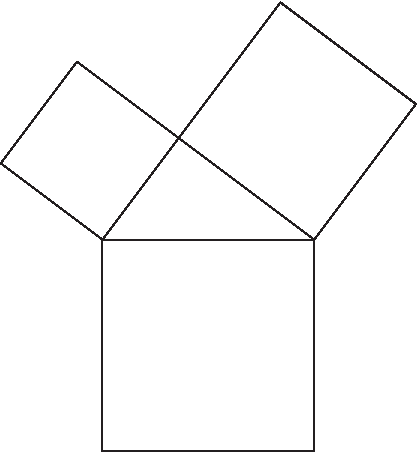
\includegraphics[width=200pt]{pitagora}
\caption[teor. di Pitagora]{Triangolo rettangolo}
\label{figura:pitagora}
\end{center}
\end{figure}

Esistono anche modi per far girare i testo attorno alle
figure. Chi vuole consulti i manuali.

Osservate comunque che in questo stile i paragrafi nelle dimostrazioni non hanno rientro\index{paragrafi, rientro dei} e c'è un quadratino\index{dimostrazioni, quadratino di fine} alla fine.
\end{proof}

\begin{definizione}\label{def:liminfinito}
Si dice che la successione reale $x_n$ tende\index{limite di successioni}\index{successioni, limite di} a~$+\infty$ se per ogni~$M\in\R$ esiste $n_M\in\N$ tale che per ogni~$n\ge n_M$ si ha che $x_n\ge M$.
\end{definizione}

Possiamo riferirci alla definizione~\ref{def:liminfinito}
tramite la sua etichetta\index{etichette}. Il riferimento sarà ``cliccabile'' se si è caricato il pacchetto \verb!uniudtesi! (il quale chiama a sua volta \verb!hyperref!.\index{ipertesto})

\section{Formule}

Anche le formule si possono etichettare:
\begin{equation}
  \label{eq:binomio}
  a+b\,.
\end{equation}
La formula precedente dovrebbe essere la~\ref{eq:binomio} (cliccabile). Non è obbligatorio numerare tutte le formule. Le formule non numerate\index{numerazione formule}\index{formule, numerazione delle}\index{numerazione delle formule} si ottengono o con doppi dollari\index{dollari, doppi}:
$$\dot x\quad
  \ddot x\quad
  \dddot x\quad
  \ddddot x$$
o con l'asterisco\index{asterisco}:
\begin{equation*}
  \overset{\circ}{A}\quad
  \overset{*}{X}\quad
  \vec{x}
\end{equation*}
Testo\index{formula, testo nella}\index{testo nella formula} mescolato a una formula:
\begin{equation}
  x+y=1\text{ quindi }(x+y)^2=1
\end{equation}
$$(x+y)^2\ge0\quad\text{ per ogni }x,y\in\R$$
Carattere grassetto\index{grassetto matematico} matematico:
$$\boldsymbol{y}
  $$
Allineamento\index{allineamento delle formule}\index{formule, allineamento delle} di formule e tre modi di indicare la congruenza\index{congruenze} modulo~$n^2$, con la seconda e terza formula numerate\index{formule, numerazione delle}\index{numerazione delle formule}:
\begin{align}
     u & \equiv  v+1 \pmod{n!}\nonumber \\
     u & \equiv v+1 \mod{n^2} \\
     u & \equiv v+1 \pod{n^2}
  \end{align}
Una formula spezzata\index{formula, spezzamento su righe diverse}\index{spezzamento di una formula su righe diverse} su due righe, ma trattata come un tutt'uno per il numero\index{formule, numerazione delle}\index{numerazione delle formule} di formula:
\begin{equation}
  \begin{split}
    f(x)  :={}& \int_0^{+\infty}t^{x-1}e^{-t}\,dt+\\
         &{}+e^{-x}
  \end{split}
\end{equation}
Due modi di scrivere le frazioni\index{frazioni}:
\begin{equation}
  \frac{1}{2}
  \quad\frac{1}{2}\,.
  \end{equation}
Una definizione per casi\index{casi, definizione
per}\index{definizione per casi}:
\begin{equation}
  f(x):=
  \begin{cases}
    x^2 & \text{se } x\ge0 \\
   -x^2 & \text{se }x<0
  \end{cases}
\end{equation}
Matrici\index{matrici} con e senza parentesi\index{parentesi}:
\begin{equation*}
  \begin{matrix}
    0 & 1 \\
    1 & 0
  \end{matrix}\quad
  \begin{pmatrix}
    0 & 1 \\
    1 & 0
  \end{pmatrix}
  \quad
  \begin{vmatrix}
    0 & 1 \\
    1 & 0
  \end{vmatrix}
\end{equation*}
Due formule di seguito senza allineamento\index{formule, allineamento delle}\index{allineamento delle formule}:
\begin{gather}
  (a+b)^2=a^2+2ab+b^2\label{eq:quadrato} \\
  (a+b)(a-b)(a^2+b^2)=a^4-b^4
\end{gather}

Un esempio di tavola\index{tavola}:

\begin{center}
\begin{tabular}{||l|lr||} \hline
gnats & gram & \$13.65 \\ \cline{2-3}
      & each &      .01 \\ \hline
gnu   & stuffed & 92.50 \\
    \cline{3-3}
emu   &      & 33.33 \\ \hline
armadillo & frozen & 8.99 \\ \hline
\end{tabular}
\end{center}